\documentclass{article}
\usepackage[utf8]{inputenc}
\usepackage[english]{babel}
\usepackage{graphicx}

\usepackage[en-US]{datetime2}
\usepackage{minted}
\usemintedstyle{solarizedlight}

\usepackage{cleveref}
\usepackage{hyperref}

\title{Milestone 1 Evaluation\\
{\small CSE 232B, UC San Diego, Spring Q 2015}}
\author{Jens Emil Gydesen\thanks{UCSD SID: Ublah} \and
        Martin Bjeldbak Madsen\thanks{UCSD SID: U6616356}}
\date{\DTMdisplaydate{2015}{5}{13}{3}, \DTMdisplaytime{11}{10}{00}}

\begin{document}
\maketitle

\section{Query 1}
Finds act, scene and speaker of famous line \emph{Et tu, Brute! Then fall, Caesar}. Should return 

\begin{minted}{xml}
<result>
  <who>CAESAR</who>
  <when>
    <act>ACT III</act>
    <scene>
      SCENE I.  Rome. Before the Capitol; the Senate sitting above.
    </scene>
  </when>
</result>
\end{minted}

\subsection{Query}
\begin{minted}{xquery}
<result>{
for $a in doc("j_caesar.xml")//ACT,
    $sc in $a//SCENE,
    $sp in $sc/SPEECH
where $sp/LINE/text() = "Et tu, Brute! Then fall, Caesar."
return <who>{$sp/SPEAKER/text()}</who>,
       <when>{<act>{$a/title/text()}</act>,
             <scene>{$sc/title/text()}</scene>}
       </when>
}</result>
\end{minted}

\subsection{Parse Tree}
See \cref{fig:parseTree1}.
\begin{figure}[htpb]
  \centering
  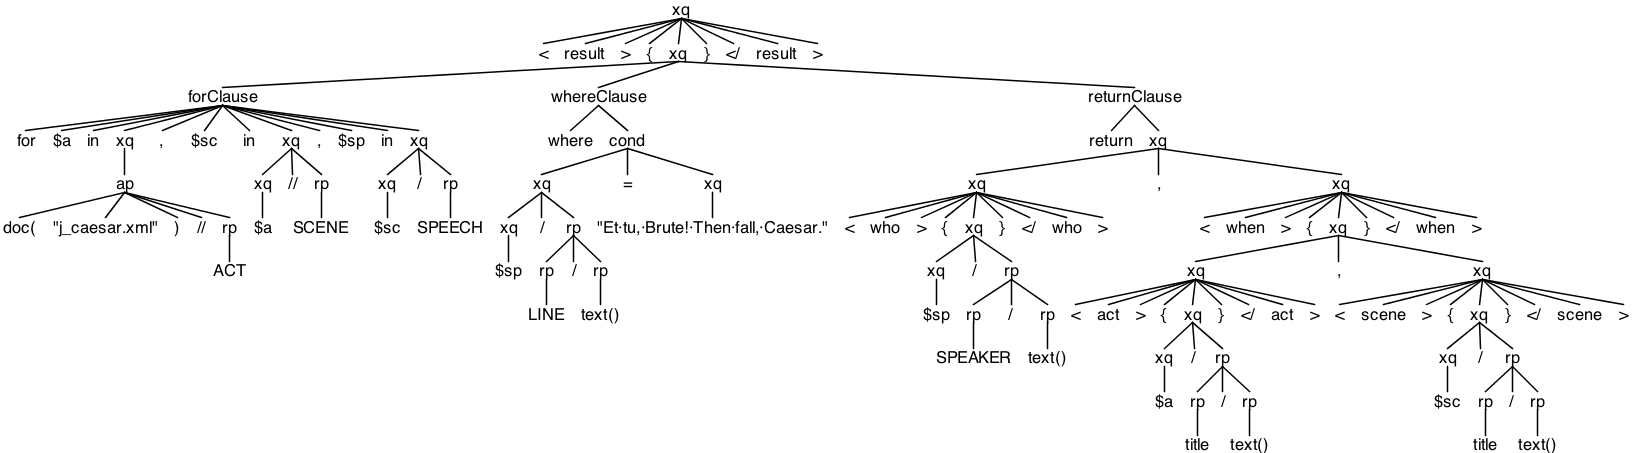
\includegraphics[width=\linewidth]{imgs/antlr4_parse_tree_query_1.png}
  \caption{Parse tree for the first query.}\label{fig:parseTree1}
\end{figure}

\subsection{Output}

\section{Query 2}
Groups all acts by speaker, that is, return a list of elements of type element  \texttt{speaks \{ element who \{String\}, (element when \{String\})+ \}}, where the String contents of the \texttt{<who>} element is a speaker name, and the contents of the \texttt{<when>} elements are act names.

\subsection{Query}
\begin{minted}{xquery}
for $s in doc("j_caesar.xml")//SPEAKER
return <speaks>{<who>{$s/text()}</who>,
                for $a in doc("j_caesar.xml")//ACT
                where some $s1 in $a//SPEAKER satisfies $s1 eq $s
                return <when>{$a/title/text()}</when>}
       </speaks>
\end{minted}

\subsection{Parse Tree}
See \cref{fig:parseTree2}.
\begin{figure}[htpb]
  \centering
  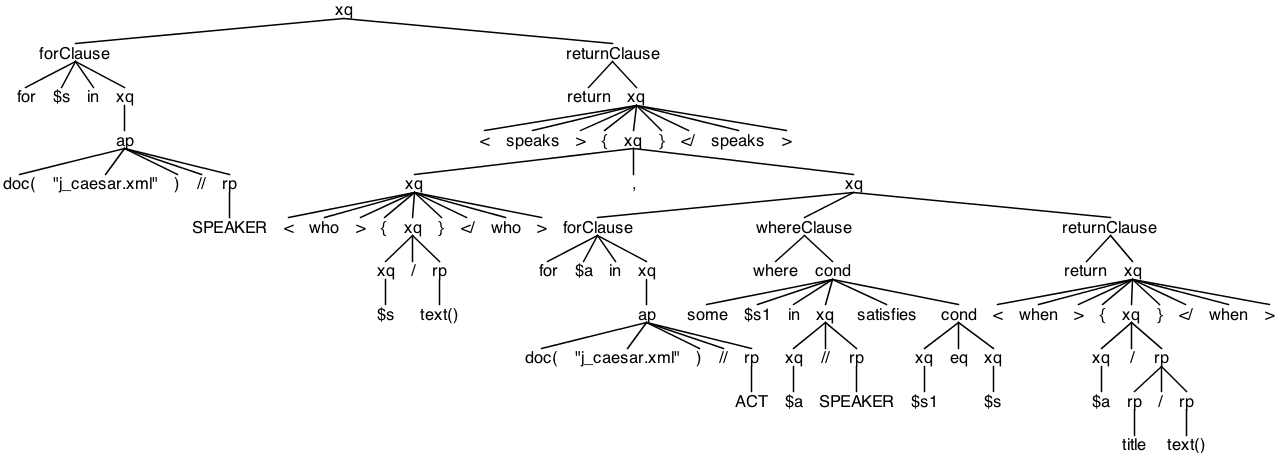
\includegraphics[width=\linewidth]{imgs/antlr4_parse_tree_query_2.png}
  \caption{Parse tree for the second query.}\label{fig:parseTree2}
\end{figure}

\subsection{Output}

\end{document}
